\chapter{First-hitting-time models}

\section{Survival data}
Time to event data are seen in many different contexts, including medicine, engineering, biology, and sociology.
One considers a set of individuals $i$, $i=1,2,\ldots,N$, for which an event can happen.
The term \textit{survival data} is used to refer to time to event data where such events only can happen once.
An overview of modelling of survival data can be found in for example \citet{ABG}.
Althought the term survival data sounds like it refers to deaths only, the event in question may be anything of interest.
%Large Important applications in biomedical statistics, where we are often interested in, for example, the factors contributing to why some cancer patients recover, and others experience recurrence.
%\subsection{General idea}
You might, for example, be a doctor performing a study of cancer patients, and monitoring them for possible relapse.
In this case, the event is the relapse.
Or, possibly, you are a demographer looking at all parents who have only one child, and you are monitoring the time that elapses before they have a second child.
Clearly, to observe such data in real life, we must wait until the event actually happens.
This might in some cases never happen, or it might take a very long time.
Consider, for example, a clinical trial of $N$ patients who have been treated for some disease, and where $T_i$, $i=1,\ldots,N$, is the time until their relapse.
Such a trial can only last a certain amount of time, say, until a time $\tau$.
Luckily, not every patient relapses during that time, and so the actual time to their relapse, $\tilde{T}_i$, is not observed.
%Note that it might turn out that the actual $\tilde{T}_i$ does not exist.
We could throw away these observations without an observed event, and consider them irrelevant.
But we at least know that these patients survived until time $\tau$.
We therefore work with the concept of incomplete data, which we call \textit{censored} survival data \citep{ABG}.

\subsection{Independently censored survival data}\label{subsec:survdata}
The time-to-event $\tilde{T}$ is a random variable of a non-negative domain.
This time-to-event has a corresponding random variable $W$ which represents the censoring time of the time-to-event.
The observed, and possibly censored, survival time is
\begin{equation*}
    T=\min(\tilde{T},\,W).
\end{equation*}
We also operate with a corresponding censoring indicator
\begin{equation*}
    D=\indicator(\tilde{T}=T),
\end{equation*}
which is 1 if the observed survival time is not censored, and 0 if it is.
In the clinical trial example mentioned, the censoring time $W$ would be the end of the possible observation period of the trial, namely $\tau$.
An important property of survival data is the concept of \textit{independent censoring}, also called \textit{random censoring}.
We say that we have independent censoring if the censoring indicator $D$ is independent of the time, meaning that
\begin{equation*}
    P(T|D)=P(T).
\end{equation*}
What we have so far called censored data is in truth \textit{right-censored} survival data.
Left-censoring is also possible, but we will not discuss it in this thesis, and so we continue to simply use the term ``censoring.''

\subsection{The survival function $S(t)$, the hazard function $\hz(t)$, and their estimators}
When studying censored survival data, we are interested in estimating the probability of surviving until time $t$, which is called the survival function, and is defined as
\begin{align*}
    S(t)=\Pr(T>t)=1-\Pr(T<t)=1-F(t).
\end{align*}
Here $F(t)$ is the familiar cumulative distribution function.
If the derivative of $F(t)$ exists, we denote it $f(t)$, and then the lifetime $T$ has probability distribution function (pdf) $f(t)$.

Another function we are interested in is the hazard function.
This is the probability of the event happening at time $t$, conditioned on the event not having happened yet.
More formally, the hazard function is defined as
\begin{equation*}
    \hz(t)=\lim_{\epsilon\to0}\frac{\Pr(T<t+\epsilon|T>t)}{\epsilon}.
\end{equation*}
Estimating the hazard function is hard, and we do not achieve the usual $\sqrt{n}$ convergence.
\todo[inline]{Find and add citation.}
It is, however, typically the function we are most interested in, as we will see later, in subsection \ref{subsec:ph-reg}.
Note that by observing
\begin{equation*}
    \Pr(T<t+\epsilon|T>t)=\frac{\Pr(T<t+\epsilon,T>t)}{\Pr(T>t)}=\frac{F(t+\epsilon)-F(t)}{S(t)},
\end{equation*}
and inserting this into the hazard function we have the relation
\begin{equation}
\label{eq:hfs}
    \hz(t)=\frac{1}{S(t)}\lim_{\epsilon\to0}\frac{F(t+\epsilon)-F(t)}{\epsilon}=\frac{f(t)}{S(t)}=\frac{-S^\prime(t)}{S(t)},
\end{equation}
where the probability distribution function $f(t)$ is obtained by its limit definition, and we note that $S^\prime(t)$ is the derivative of $1-F(t)$, which is $-f(t)$.
We further note that by interchanging the notation for derivation, we obtain
\begin{equation}\label{eq:alpha-diff}
\alpha(t)=\frac{S^{\prime}(t)}{S(t)}=\frac{\frac{\d S}{\d t}}{S(t)}.
\end{equation}
By integrating the hazard from 0 to time $t$, we get the cumulative hazard function,
\begin{equation}\label{eq:cumulative-hazard-1}
    A(t)=\int_0^t\hz(s)\d s,
\end{equation}
and we insert \eqref{eq:alpha-diff} into \eqref{eq:cumulative-hazard-1},
\begin{equation}\label{eq:cumulative-hazard}
\begin{split}
     A(t)=-\int_0^t\frac{\frac{\d S}{\d s}}{S(s)}\d s=-\int_0^t\frac{1}{S(s)}\d S=-\log(S(t)),
\end{split}
\end{equation}
which is an important relationship.
Given survival data $(t_i,d_i)_{i=1}^N$, we introduce the \textit{risk set} $R(t)$, which gives the set of all individuals at risk at time $t$,
\begin{equation*}
    R(t)=\{i\colon t_i\geq t\}.
\end{equation*}
We further introduce the function $Y(t)$, which is equal to the number of individuals still at risk at time $t$,
\begin{equation*}
    Y(t)=\#R(t)=\#\{i\colon t_i\geq t\},
\end{equation*}
where $\#(\cdot)$ is the counting operator over a set.
Note that $Y(t)$ does not depend on the censoring indicators, since an individual is at risk at time $t$ even though it turns out that it did not die, i.e., its censoring indicator $d_i$ is 0.
Estimating the survival function $S(t)$ is usually done by the Kaplan-Meier estimator \citep{kaplan-meier},
\begin{equation*}
    \hat{S}_{\text{KM}}(t)=\prod_{i:\{t_i\leq t\}}1-\frac{d_i}{Y(t_i)},
\end{equation*}
and the cumulative hazard function $A(t)$ by the Nelson-Aalen estimator \citep{nelson, aalen1978},
\begin{equation*}
    \hat{A}(t)=\sum_{i:\{t_i\leq t\}}\frac{d_i}{Y(t_i)}.
\end{equation*}

\section{Classical inference approaches}
\subsection{Likelihood regression}
Consider survival data $(t_i,d_i),\,i=1,2,\ldots,N$, where $t_i$ is the time to event of individual $i$, and $d_i$ is a censoring indicator of the usual type, meaning it is 1 if the event has been observed, and 0 if not.
To make inference on what affects the time to event, we need to consider covariates.
Covariates are information about an individual.
In medical applications, typical covariates are age, gender, disease status, as well as clinical measurements.
Denote the covariates, i.e., the information, of an individual $i$ by $x_{i,1},x_{i,2},\ldots,x_{i,p}$, where $p$ is the total number of pieces of information.
We gather these in a vector $\x_i=(x_{i,1},x_{i,2},\ldots,x_{i,p})$.
We may now consider a data set of complete tuples of survival data with covariates,
\begin{equation}\label{eq:surv-D}
    D=(t_i,d_i,\x_i)_{i=1}^N.
\end{equation}
Now, consider a survival time distribution
\begin{equation}\label{eq:surv-time-dist}
    \psi(\bbeta),
\end{equation}
which has a vector of regression parameters $\bbeta=(\beta_1,\beta_2,\ldots,\beta_p)$, with one parameter $\beta_j,\,j=1,2,\ldots,p$ corresponding to one covariate $x_j$.
This distribution has a parameterized survival function
\begin{equation*}
    S(t|\bbeta,\x)
\end{equation*}
and a parameterized probability distribution function
\begin{equation*}
    f(t|\bbeta,\x).
\end{equation*}
Given an observed dataset $D$ \eqref{eq:surv-D}, we wish to make inference on which covariates affect the survival time.
One way to do this, having assumed a specific survival distribution $\psi(\bbeta)$, is to construct a so-called (joint) likelihood.
The likelihood is a function of the parameters $\bbeta$ in the distribution, given the observed sample.
The likelihood is maximized at the parameters which have the highest probability of yielding the observed sample.
If all censoring indicators are 1, meaning all observations are actual events, we are in the usual statistical regression landscape.
For each observation, its likelihood is the probability of observing its event at $t_i$ given the parameters and the data,
\begin{equation*}
    f(t_i|\bbeta,\x_i).
\end{equation*}
A typical assumption when setting up a (joint) likelihood is to assume that the conditional distribution of each observation is independent and identically distributed (\textit{iid}), given the data.
Hence the joint likelihood is the product of all the single likelihood contributions,
\begin{equation*}
    L(\bbeta)=\prod_{i=1}^N f(t_i|\bbeta,\x_i).
\end{equation*}
But we need to consider the case of censored survival data, and we wish to set up a joint likelihood for such a data set.
Again assume that the observations $D=\{\x_i,y_i\}_{i=1}^N$ are independent and identically distributed from a survival distribution $\psi(\bbeta)$.
In the case of an uncensored observation $i$, meaning $d_i=1$, the single contribution to the likelihood is
\begin{equation}\label{eq:f}
    f(t_i|\bbeta,\xi)
\end{equation}
to the likelihood.
If the event has not occurred, i.e. the observation is censored, $d_i$ is 0.
In this case, we do not have the actual lifetime, and so we cannot use the lifetime distribution, but we must instead use the survival distribution.
After all, the fact that this individual is alive at time $t_i$ is informative.
Therefore this observation contributes
\begin{equation}\label{eq:S}
    S(t_i|\bbeta,\xi)
\end{equation}
to the likelihood.
Since an observation can only be either censored or not censored at the same time, $d_i$ is either 0 or 1.
This means that we can combine expressions \eqref{eq:f} and \eqref{eq:S} in a way that a single observation contributes the product
\begin{equation*}
    f(\ti|\x_i)^{d_i}S(\ti|\x_i)^{1-d_i}
\end{equation*}
to the likelihood.
Since we assume the observations to be independent, the likelihood is, again, the product of the single complete contributions.
The complete likelihood becomes
\begin{equation}\label{eq:surv-lik}
    L(\bbeta)=\prod_{i=1}^N f(t_i|\x_i,\bbeta)^{d_i} S(t_i|\x_i,\bbeta)^{1-d_i}.
\end{equation}
It is more convenient to work with the log likelihood,
\begin{align}\label{eq:surv-log-lik-1}
\begin{split}
    l(\bbeta)&=\log L(\bbeta) \\
    &=\sum_{i=1}^N\left[ d_i \log f(t_i|\x_i,\bbeta) + (1-d_i)\log S(t_i|\x_i,\bbeta)\right].
\end{split}
\end{align}
Note that since $A(t)=-\log S(t)$ and $f(t)=\alpha(t)S(t)$, see \eqref{eq:cumulative-hazard} and \eqref{eq:hfs}, respectively, \eqref{eq:surv-log-lik-1} further simplifies to
\begin{equation*}%\label{eq:surv-log-lik-2}
    l(\bbeta)=\sum_{i=1}^n\left[ d_i \log \hz(t_i|\x_i,\bbeta) - A(t_i|\x_i,\bbeta)\right].
\end{equation*}
For any survival distribution $\psi(\bbeta)$ \eqref{eq:surv-time-dist} for which either form of $l(\bbeta)$ can be calculated, we can perform maximum likelihood estimation of its parameters.

\subsection{Proportional hazards regression}\label{subsec:ph-reg}
In other fields of statistics, we are often most interested in modelling the probability distribution function and the cumulative distribution function.
In survival analysis, however, we are typically more interested in modelling the hazard function.
In this subsection, we consider the effect of covariates on the hazard function $\hz(\cdot)$.
How may we use a covariate vector $\x$ in modelling the hazard rate?
A very common model to choose here is a proportional hazards model, which assumes
\begin{equation}\label{eq:PH}
    \hz(t|\x)=\hz_0(t)r(\x|\bbeta),
\end{equation}
where $\hz_0(t)$ is an \textit{unspecified} baseline hazard function shared between all individuals, and $r(\x|\beta)$ is a so-called relative risk function parameterized with regression coefficients $\bbeta=(\beta_1,\ldots,\beta_p)$. We choose $r(\x)$ such that it is appropriately normalized, meaning $r(\0)=1$.
A crucial assumption here is that the effects of the covariates are fixed in time. In this setup, it turns out that we can do regression without specifying the baseline hazard. This is a major advantage, because we then do not have to think about modelling effects in time. Given data $D=(t_i,d_i,\x_i)_{i=1}^N$, we may set up a so-called partial likelihood \citep{cox-model}.

The idea behind the partial likelihood is as follows.
We have observed data $D$ with at least some censoring indicators $d_i$ equal to 1.
In partial likelihood regression, we simply ignore the censored observations.
Informally, the probability of the event happening at a time $t$ for some individual $j$ is the probability of an event happening to individual $i$ at time $t$, divided by the total probability of an event happening at time $t$, the instantaneous probability of an event happening to that individual at that time, i.e., the hazard function of that individual at that time,
\begin{equation}\label{eq:hazard-frac-informal}
    \frac{\Pr(\text{event happens to individual }i\text{ at time }t)}{\Pr(\text{event happens to \textit{any} individual }j\text{ at time }t)}.
\end{equation}
More formally, we look at the instantaneous probability of an event happening for the individual $i$, which is the hazard function $\hz(t|\x_i)$.
Thus the total probability of an event happening at time $t$ is the sum of the hazard functions of all individuals in the risk set
$R(t)$, which, again, is defined as
\begin{equation*}
    R(t)=\{i\colon t_i\geq t\,,i=1,2,\ldots,n\}.
\end{equation*}
From all the uncensored observations, we know that events happened at times $\{t_i\colon d_i=1,\,i=1,2,\ldots,N\}$. Therefore, we can construct expressions for \eqref{eq:hazard-frac-informal} at all the observed, uncensored, times.
Inserting the probabilities into the informal expression in \eqref{eq:hazard-frac-informal}, an individual with an observed event at $t_i$ 
contribues to the likelihood with
\begin{equation}\label{eq:hazard-frac}
    \frac{\hz_0(t_i)r(\x_i)}{\sum_{j\in R(t_i)} \hz_0(t_i)r(\x_j)}.
\end{equation}
Now, assuming that observations are independent and identically distributed, we say that the \textit{partial likelihood} of the model
given the observed data is the product of all ratios \eqref{eq:hazard-frac}, namely
\begin{equation}\label{eq:pl}
    \pl(\bbeta)=\prod_{i\colon d_i=1}\frac{\hz_0(t_i)r(\x_i)}{\sum_{j\in R(t_i)} \hz_0(t_i)r(\x_j)}=\prod_{i\colon d_i=1}\frac{\hz_0(t_i)r(\x_i)}{\hz_0(t_i)\sum_{j\in R(t_i)}r(\x_j)}.
\end{equation}
In the expression above, \eqref{eq:pl}, we rearrange the denominator such that the baseline hazard of individual $i$, $\hz_0(t_i)$, is moved out of the sum.
This hazard depends on individual $i$, while the sum is a sum over all individuals $j$.
It therefore cancels out, and we are left with just the relative risk functions,
\begin{equation*}
    \pl(\bbeta)=\prod_{i\colon d_i=1}\frac{r(\x_i)}{\sum_{j\in R(t_i)}r(\x_j)}.
\end{equation*}
The fact that the baseline hazard cancels out is quite powerful.
Even though proportional hazards regression is not fully parametric,
the canceling means that we can model the effect of covariates in a fully parametric way, and without having to consider the baseline hazard.

Consider now possible choices for the relative risk function $r(\x)$.
The most common choice, by far, for $r(\x)$ is
\begin{equation*}
    r(\x)=\exp(\x^T\bbeta),
\end{equation*}
which leads to the famous Cox model \citep{cox-model}.
The Cox model is an attractive model because the value of the parameter $\bbeta$ has a nice interpretation.
Assume we have two observations with covariate vectors $\x_1$ and $\x_2$, and that $\x_2$ is equal to $\x_1$ except for in element $j$, where $x_{2j}=x_{1j}+1$.
Then the ratio of the two hazard rates becomes
\begin{equation*}
    \frac{\exp(\x_2^T\bbeta)}{\exp(\x_1^T\bbeta)}=\exp((\x_2-\x_1)^T\bbeta)=\exp(\beta_j).
\end{equation*}
Furthermore, if the two covariate vectors differ in more elements, say, that, each element in $\x_2$ is one unit increased from each element in $\x_1$, we get that
\begin{equation*}
    \frac{\exp(\x_2^T\bbeta)}{\exp(\x_1^T\bbeta)}=\exp((\x_2-\x_1)^T\bbeta)=\exp(\beta_1+\beta_2+\ldots+\beta_p)=\exp(\beta_1)\exp(\beta_2)\cdots\exp(\beta_p).
\end{equation*}
In other words, each unit increase in a covariate is a multiplicative factor in the hazard.
Cox regression is used very much in applied research.
%We will here give a simple example to illustrate its use.

%\subsection{Cox regression example}
%Lorem ipsum.

\subsection{Issues with the proportional hazards assumption}
When assuming \eqref{eq:PH}, i.e. $\hz(t|\x)=\hz_0(t)r(x|\bbeta)$, we are making a relatively strong assumption.
Namely, we assume that the ratio between the hazard function of two individuals is the same \textit{at all times}, because the part of $\hz(t|\x)$ cancels out when we do regression, and because we assume that the covariate effects are constant in time, as $r(x|\bbeta)$ is not a function of time.
This assumption goes under the name of the proportional hazards (PH) assumption.
While, as we saw, this assumption greatly simplifies the inference, it is not necessarily satisfied in practice.
In any case, it is very difficult to verify, in case of multivariate analysis, especially in high-dimensional contexts.
In the literature, there exist alternative models, that do not require the PH assumption.
One of these is Aalen's additive model, which is an example of additive hazard modelling.
In Aalen's model, the hazard function takes the form
\begin{equation*}
    \alpha(t|\x)=\beta_0(t)+\beta_1(t)x_1(t)+\beta_2(t)x_2(t)+\ldots+\beta_p(t)x_p(t),
\end{equation*}
where $\beta_j(t),j=1,\ldots,p$ is the increase in the hazard at time $t$ corresponding to a unit's increase in the $j$-th covariate. Another alternative model to the Cox model is the first hitting threshold model.
In this thesis we will focus on the latter, focusing on the analysis of high-dimensional data.
To our best knowledge, this is the first study which tries to combine FHT models and high-dimensional data.

\subsection{Cox, proportional hazards, and variable selection}
The PH assumption \eqref{eq:PH} is very often not valid.
Consider survival data with two covariates $x_1$ and $x_2$.
With Cox regression, the hazard is
\begin{equation*}
    \alpha(t|x_{i,1},\,x_{i,2})=\alpha_0(t)\exp(\beta_1x_{i,1}+\beta_2x_{i,2}).
\end{equation*}
There is a model inconsistency problem here.
If we only observe $x_{i,1}$, and calculate the hazard $\alpha(t|x_{i,1})$, then this will not be of Cox regression form, regardless of the distribution of $x_2|x_1$.

In addition, if there is perfect Cox structure given $x_1$ alone, and perfect Cox structure given $x_2$ alone, one almost never has a Cox model in the joint space $(x_1,\,x_2)$.
That is, one almost never has the proportional hazards assumption actually satisfied.
However, in practice, Cox regression is robust and tends to work well.
\todo[inline]{Find citation for this paragraph!}

Given that Cox sometimes leaves us wanting of a more flexible and more theoretically plausible model, there is room for other models.
One may attempt to start the model building task at a deeper level, taking biologically plausible assumptions about the background processes associated with life lengths.
This is where first-hitting-time models come in.

\section{First hitting time models}\label{sec:FHT}
So far we have done regression by modelling the log-likelihood $l(\cdot)$ and the hazard rate $\hz(\cdot)$.
Therefore we have not thought much about how a time-to-event is \textit{generated}, other than the fact that it arises from a survival distribution $S(\cdot)$ with a corresponding hazard function $\hz(\cdot)$.
In this context, an individual is alive at one time.
Slightly later, it is either still alive, or it may have died.

Instead, another way to approach survival analysis is to model the process which generates the survival data.
We can imagine that each individual has an underlying stochastic process $Y(t)$, which we call a health process.
When this health process reaches a barrier, or an end state, the individual dies.
This is a conceptually appealing framework:
Instead of just being a stochastic lifetime with a binary status of an event having happened or not or alive, it introduces the concept of distance to the event.
We may call the time the health process hits the barrier or the end state the \textit{first hitting time} (FHT) of a boundary or threshold state, by sample paths of a stochastic health process.
This health process may be observable, but for most purposes it will be latent, i.e., unobservable.

Many types of time-to-death data may, in fact, be interpreted as FHTs.
FHT models have a long history of application in diverse fields, including medicine and engineering.
They have been used to describe the length of a hospital stay \citep{whitmore1975,eaton-whitmore}, to model the duration of a strike \citep{lancaster}, to estimate degradation in components \citep{whitmore1995}, and to assess lung cancer risk in railroad workers \citep{leewhitmore2004}.

\citet{eaton-whitmore} discuss FHTs as a general model for hospital stay.
\citet{aalengjessing2001} provide an overview of much of this subject.
\citet{lawless2011} provides a compact overview of the theory.
\citet{leewhitmore2004a} provides an overview of first hitting time models for survival and time-to-event data.
There is a large literature dealing with theoretical and mathematical aspects of FHT models.

Models based on this view are called first hitting time models (FHT).
FHT models were introduced in \citet{whitmore1986}, see \citet{leewhitmore2006} for a complete overview.
Note that these authors use the term threshold regression when referring to regression for first hitting time models.
We have, following \citet{caroni2017}, chosen to not use this term, as it is also used to refer to a well established, and quite different, topic in econometrics.

\subsection{General idea}\label{fht-idea}
A first-hitting-time (FHT) model has two basic components:
\begin{enumerate}
\item A parent stochastic process $\{Y(t),\,t\in\setT,\,y\in\setY\}$, with initial value $Y(0)=y_0$, where $\setT$ is the time space and $\setY$ is the state space of the process.
\item A boundary set $\setB$, where $\setB\subset\setY$. This is at times also referred to as a barrier or a threshold, depending on which is most appropriate to the context.
\end{enumerate}
The process $\{Y(t)\}$ may have a variety of properties, such as one or many dimensions, the Markov property, continuous or discrete paths, and monotonic sample paths. Whether the sample path of the parent process is observable or latent (unobservable) is an important distinguishing characteristic of the FHT model. Latent (unobservable) processes are the most common by far. The boundary set $\setB$ may also have different features. The basic model assumes that $\setB$ is fixed in time.
Some applications may require dependencies on time, i.e., $\setB(t)$, but this case will not be considered in this thesis, and so we write $\setB$.

Taking the initial value $Y(0)=y_0$ of the process to lie outside the boundary set $\setB$, the \textit{first hitting time} of $\setB$ is the random variable $T$ defined as
\begin{equation}\label{eq:fht-t}
    T=\inf_t\left(t\colon Y(t)\in\setB\right).
\end{equation}
Thus, the first hitting time is the time when the stochastic process first encounters the boundary set $\setB$. The boundary set defines a stopping condition for the process. Note that when the parent process is latent, there is no direct way of observing the FHT even in the state space of the process.

In some versions of the FHT model, there is no guarantee that the process $\{Y(t)\}$ will reach the boundary set $\setB$, so $P(T<\infty)<1$. We will let $T=\infty$ denote the absence of a finite hitting time with
\begin{equation}\label{eq:T-is-infinity}
    P(T=\infty)=1-P(T<\infty).
\end{equation}
This condition is sometimes plausible and a desirable model feature.
Two common concepts in survival analysis might lead to this.
One is the case of competing risks.
That is the case where an individual might die from not only one, but several causes, but we are only studying one of these.
Naturally, then, we would not except that all individuals die from the cause that we study, and hence $P(T<\infty)<1$.
The second concept is related to ``cure models.''
A cure model is a model where there are individuals with zero frailty, i.e., a nonsusceptible group \citep{ABG}.
Consult \citet{maller1996survival} for more details.

\subsection{Examples of first-hitting-time models}
The parent stochastic process $Y(t)$ may take many forms, from Wiener processes to Markov chains.
Similarly, the boundary state may also take various forms.
For example, it may be a fixed threshold in a Wiener process or an absorbing state in a Markov chain.
The freedom in the choice of these quantities show how flexible the FHT framework is.
The choice of boundary must fit the process, such that the boundary set is a subset of the state space.
We will now briefly mention some examples of choices of health processes and corresponding boundaries, before focusing on the most studied case, which uses as a choice of health process the Wiener process.
These examples are taken from \citet{leewhitmore2006}.
\begin{enumerate}
    \item
        \textit{Bernoulli process and negative binomial first hitting time.}
        The number of trials $S$ required to reach the $m$-th success in a Bernoulli process $\{B_t,t=1,2,\ldots\}$ has a negative binomial distribution with parameters $m$ and $p$, where $p$ is the success probability of each trial. To give this setup our standard representation, we consider a parent process
        \begin{equation*}
            \{Y(t),\,t=0,1,2,\ldots\}
        \end{equation*}
        with initial value $Y_0=y_0=m$ and let
        \begin{equation*}
            Y_t=y_0-B_t,\,t=1,2,\ldots,
        \end{equation*}
        where $\{B_t\}$ is the aforementioned Bernoulli process. The first hitting time is the first Bernoulli trial $t=T$ for which $Y_t$ equals 0. The number of rocket launches to get $m$ satellites in orbit is an example of this FHT model.
    \item
        \textit{Gamma process and inverse gamma first hitting time.}
        Consider a parent process
        \begin{equation*}
            \{Y(t),\,t\leq0\}
        \end{equation*}
        with initial value $Y(0)=y_0>0$. Let
        \begin{equation*}
            Y(t)=y_0-Z(t),
        \end{equation*}
        where $Z(t),\,t\leq0$ is a gamma process with a scale parameter $\beta$, a shape parameter $\alpha$ and a starting point $Z(0)=0$. The first hitting time of the zero level in the parent process ($Y=0$) has an inverse gamma cumulative distribution function (cdf), defined by the identity
        \begin{equation*}
            P(T>t)=P(Z(t)<y_0).
        \end{equation*}
        The identity follows from the fact that a gamma process has monotonic, nondecreasing sample paths.
        Computational routines for the gamma cdf allows the cdf of T to be computed readily.
        \citet{singpurwalla1995} and \citet{lawless2004} consider the gamma process as a model for degradation.
        A gamma process is a good choice if we want a monotonic restriction on the movement of the health process \citep{leewhitmore2006}. 
        It might, for example, make sense if the health process is meant to model e.g. the breakdown of a structure.
    \item
        \textit{Poisson process and Erlang first hitting time.}
        The time $S$ until the occurrence of the $m$-th event in a Poisson process
        \begin{equation*}
            \{N(t),\,t\geq 0\}
        \end{equation*}
        with rate parameter $\lambda$ has an Erlang distribution with parameters $m$ and $\lambda$.
        Again, to give this setup our standard representation, we consider a parent process
        \begin{equation*}
            \{Y(t),\,t\geq 0\}
        \end{equation*}
        with initial value $Y(0)=y_0=m$ and let $Y(t)=y_0-N(t$, where
        \begin{equation*}
            \{N(t),\,t\geq 0\}
        \end{equation*}
        is the preceding Poisson process.
        The first hitting time is the earliest time $t=S$ when $Y(t)=0$.
        This FHT model is illustrated by the time to failure of an engineering system consisting of $m$ components in parallel, having identical and independent exponential lifetimes, that are placed in service successivelu as failures occur.
\end{enumerate}
We are to choose a stochastic process to model a person's health process.
A person's health, although generally decreasing over longer periods of time, will fluctuate, at times going up, and at times going down.
If we consider the health process to be analogous with a person's health, it therefore makes sense to use a process which can both go up and down.
Therefore the choice of a gamma process as the health process would not be appropriate.

The most usual setup for a first hitting time model is to have the health process be a Wiener process, and the boundary set be a fixed threshold level.
This is attractive because it has closed-form probability and cumulative density functions, and its likelihood is computationally simple. 
There are also no restrictions on the movements of the process, meaning, it is non-monotonic.
We will first give an introduction to the Wiener process.

\subsection{Wiener process}
Consider a continuous stochastic process $W(t)$ defined for $t\in[0,\infty)$, taking values in $\R$, and with initial value $W(0)=0$. If $W$ has increments that are independent and normally distributed with
\begin{equation*}
    \E[W(s+t)-W(t)]=0\text{   and   }\Var[W(s+t)-W(t)]=s,
\end{equation*}
we call $W$ a Wiener process.
In other words, each increment has expectation 0 and has standard deviation proportional to the square root of the length of the time interval.
The position of the process at time $t$ always follows a Gaussian distribution $N(0, \sqrt{t})$ \citep{ABG}.
To increase the flexibility of the Wiener process, we can introduce a new process $Y$,
\begin{equation}\label{wiener}
    Y(t)=y_0+\mu t+\sigma W(t),
\end{equation}
which is called a Wiener process with initial value $y_0$, drift coefficient $\mu$, and diffusion coefficient $\sigma$.
A good introduction to Wiener processes can be found in \citet{cox1965}.

\subsection{Wiener process as health process causes an inverse Gaussian first hitting time}
If we choose the stochastic process to be a Wiener process with intercept and drift \eqref{wiener}, and we let the boundary be the non-positive numbers, $\setB=(-\infty,0]$, then \eqref{eq:fht-t} becomes
\begin{equation*}
    T=\min_t\left(t\colon Y(t)<0\right),
\end{equation*}
i.e. the first hitting time is the time it takes for the process to first reach a non-positive value.
(Note that since the Wiener process is continuous, there is no difference between $\leq$ and $<$. We therefore use $<$ for convenience.)
It can be shown that the first hitting time of such a Wiener process follows an inverse Gaussian distribution \citep{chhikara1988}, with probability distribution function (pdf)
\begin{equation}
\label{eq:ig-pdf}
    f(t|y_0,\mu,\sigma^2)=\frac{y_0}{\sqrt{2\pi\sigma^2t^3}}\exp\left[-\frac{(\mu t+y_0)^2}{2\sigma^2t}\right],
\end{equation}
and cumulative distribution function (cdf)
\begin{equation}
\label{eq:ig-cdf}
    F(t|\mu,\sigma^2,y_0)=\Phi\sqb*{-\frac{\mu t+y_0}{\sqrt{\sigma^2t}}}+\exp\p*{-\frac{2y_0\mu}{\sigma^2}}\Phi\sqb*{\frac{\mu t-y_0}{\sqrt{\sigma^2t}}}.
\end{equation}
As previously discussed in subsection \ref{fht-idea}, it is possible that the process does not reach the boundary set and thus cause an event.
In this case, this means that the Wiener health process never reaches 0.
This will happen if the drift $\mu$ is positive.
If so, the probability distribution function in \eqref{eq:ig-pdf} is improper, and the probability of the time not being finite is
\begin{equation}\label{eq:P-inf-FHT}
    \Pr{(T=\infty)}=1-\Pr{(T<\infty)}=1-\exp{(-2\cdot y_0\cdot\mu)},
\end{equation}
see \citet{cox1965}.

Since we in survival analysis prefer working with the survival function $S(t)=1-F(t)$ rather than the cdf $F(t)$, we note that $S(t)$ becomes
\begin{equation}
\label{eq:ig-surv}
    S(t|\mu,\sigma^2,y_0)=\Phi\sqb*{\frac{\mu t+y_0}{\sqrt{\sigma^2t}}}-\exp\p*{-\frac{2y_0\mu}{\sigma^2}}\Phi\sqb*{\frac{\mu t-y_0}{\sqrt{\sigma^2t}}},
\end{equation}
where $\Phi(x)$ is the cumulative distribution function of the standard normal,
\begin{equation*}
    \Phi(x)=\int_{-\infty}^x\phi(y)\dy,
\end{equation*}
and $\phi(x)$ is the pdf of the standard normal, defined as
\begin{equation*}
    \phi(x)=\frac{\exp\left(-x^2/2\right)}{\sqrt{2\pi}}.
\end{equation*}
Note that in \eqref{eq:ig-surv} we used the fact that the cdf of the standard normal distribution is symmetric around 0,
meaning that we were able to swap
\begin{equation*}
    1-\Phi\sqb*{-\frac{\mu t+y_0}{\sqrt{\sigma^2t}}}
\end{equation*}
with
\begin{equation*}
    \Phi\sqb*{\frac{\mu t+y_0}{\sqrt{\sigma^2t}}}.
\end{equation*}

\subsection{Effects of parameters in the Wiener process}
Let us consider a a Wiener health process where its drift $\mu$ is strictly negative, and not zero.
Such a health process will reach 0 with certainty, such that $P(T=\infty)$ \eqref{eq:T-is-infinity} is 0.
Clearly, for such a Wiener process, starting in $y_0>0$ and with a downwards drift $\mu<0$, the movement is markedly in the direction of zero.
If the variance $\sigma^2$ of the process is small in comparison to the drift, and the initial level is sufficiently large in comparison to $\sigma^2$, then the process $Y(t)$ will move in an almost straight line, such that
\begin{equation*}
    Y(t)\approx y_0+\mu t.
\end{equation*}
Consequently, the first hitting time will be a near-deterministic function of $y_0$ and $\mu$, such that
\begin{equation*}
    T\approx -\frac{y_0}{\mu}.
\end{equation*}
This is quite visible in Figure \ref{plot:wiener}, which shows examples of 5 Wiener process paths with diffusion parameter $\sigma^2=1$, initial value $y_0=10$, and drift $\mu=-1$.
Furthermore, if the diffusion is relatively small, such that $T\approx -y_0/\mu$, then either increasing $y_0$ or decreasing $\mu$ will have the same outcome, namely a larger lifetime $T$.
Conversely, either choice of decreasing the initial level or increasing the drift will cause a smaller lifetime $T$.
If $\sigma^2$ is relatively large compared to the drift, however, the diffusion part is more dominant and thus the hitting time is less predictable \citep{ABG}.

\begin{figure}
\label{plot:wiener}
\caption{Example of 5 Wiener process paths with initial value $y_0=10$ and drift $\mu=-1$.}
\centering
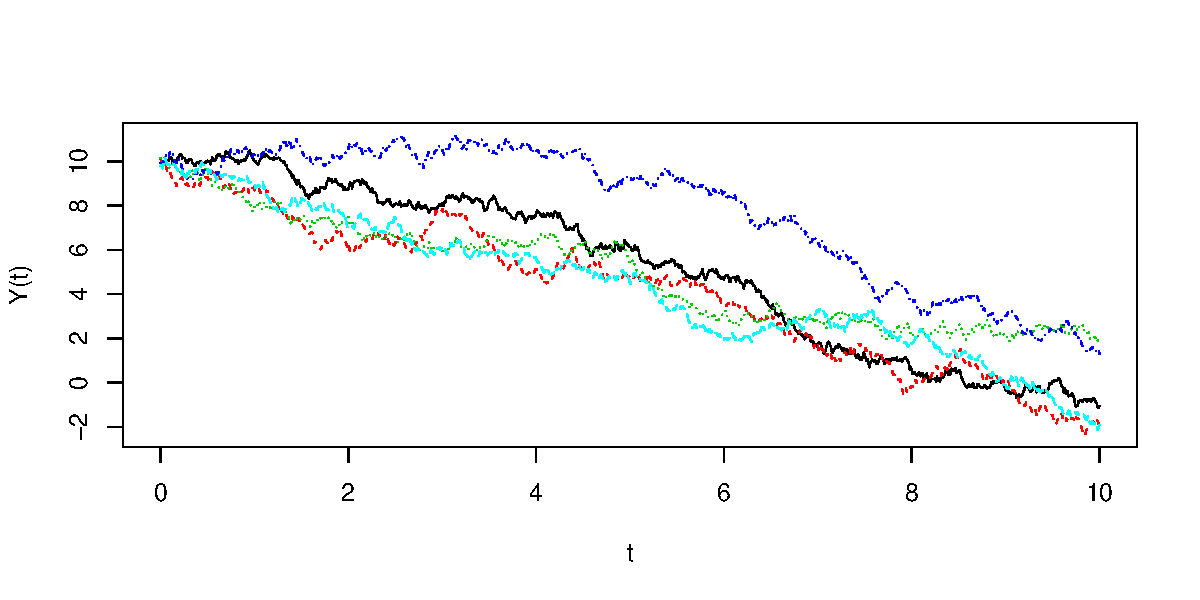
\includegraphics[scale=0.4]{figures/wiener_processes.pdf}
\end{figure}

\section{Properties of the inverse Gaussian}

\subsection{Inverse Gaussian distribution and different parameterizations}
The typical inverse Gaussian parameterization is.
\todo[inline]{Add this parameterization!}
We will use ...
This parameterization is not in the exponential family, and hence it is not a generalized linear model.

\subsection{The inverse gaussian is overdetermined if the health process is latent}
There are three parameters in the inverse Gaussian distribution, namely $y_0, \mu$ and $\sigma$.
We observe, however, that both the pdf $f(t|y_0,\mu,\sigma^2)$ in \eqref{eq:ig-pdf} and the survival function $S(t|\mu,\sigma^2,y_0)$ in \eqref{eq:ig-surv} only depend on these parameters through the ratios $\mu/\sigma$ and $y_0/\sigma$.
Hence, in reality there are only two free parameters.
In other words, we can without loss of generality fix one parameter.
The conventional way to proceed is to set $\sigma$ equal to 1 \citep{leewhitmore2006}, and in this thesis we follow this convention.

\subsection{The shape of the hazard function in the inverse Gaussian FHT model}
From \eqref{eq:hfs}, we know that the hazard function can be seen as
\begin{equation*}
    \hz(t)=f(t)/S(t).
\end{equation*}
If we plug in the inverse Gaussian versions of $f(t)$ and $S(t)$, we would get a rather intractable expression.
However, we can make some comments on its shape as it relates to different values of $y_0$ and $\mu$.
Consider the shape of the hazard rate in three different cases for the initial level $y_0$:
\begin{enumerate}
    \item
        If $y_0$ is close to zero, we essentially get a decreasing hazard rate.
    \item
        If $y_0$ is far from zero, however, we essentially get an increasing hazard rate.
    \item
        If $y_0$ is somewhat inbetween, we get a hazard rate which first increases and then decreases \citep{ABG}.
\end{enumerate}
These three examples are clearly observed in Figure ..., where we have plotted the hazard function arising from three FHT models.
All three have drift as $\mu=X$.
The first has $y_0=X$, the second has $y_0=Y$, and the third has $y_0=Z$.
\todo[inline]{add figure!}
In all three of these cases, the hazard function has a pronounced peak, which is dependent on both the initial level and the drift, of course. 
It is not as simple as the peak being at the mean lifetime, i.e., $y_0/\mu$.
Although the height of the peak will change both by changing both parameters, to simplify it a lot, $y_0$ mostly impacts at what time the
peak is, whereas $\mu$ mostly affects the height of the peak.
Regardless of the initial value, the hazard rate converges to the same limiting hazard, which is
\begin{equation*}
    \lim_{t\to\infty}\hz(t)=\frac{1}{2}\left(\frac{\mu}{\sigma}\right)^2=0.5\mu^2,
\end{equation*}
as seen in \citet{ABG}. To get an intuitive feel for this, I have made an interactive website at \verb|vegarsti.shinyapps.io/FHT_Hazard|
\todo[inline]{Add plots and more explanation here.}
%\todo[inline]{Add plots of hazard rates here. see page 401 in ABG}

\subsection{Comparison of hazard rates}
It might be of particular interest to look at the ratio between two hazard rates. We might for example look at it when the drift $\mu$ is the same, but the initial level $y_0$ is different. Then the hazard ratio is strongly decreasing. This feature is the same phenomenon as that observed in frailty models, where the relative hazards often decline \citep{ABG}.
\todo[inline]{Add plot and explain better.}
It is also of interest to do the converse, that is, look at the hazard ratio when the initial level is the same, but the drift is different. The result here is quite different.
The ratio of the hazards has a ``bathtub'' shape, which levels off at a later time \citep{ABG}.
Keep in mind here that levelling off means getting to proportional hazards.
We see that the FHT framework with a Wiener process is a highly flexible parametric model for survival analysis. Indeed, much more flexible than Cox regression, since the hazard ratios in Cox are all confined to be constant over time.
\todo[inline]{Add plot here as well; also here see ABG page 402}

\section{Regression with first-hitting-time models}\label{subsec:IG-reg}
We may introduce effects from covariates by allowing $\mu$ and $y_0$ to depend on covariates $\x$ and $\z$.
A simple and much used model \citep{leewhitmore2006, caroni2017} is to simply use the identity link function for the drift $\mu$,
\begin{equation}\label{eq:y0}
    \mu(\bbeta)=\bbeta^\T\x=\sum_{j=1}^p \beta_jx_j,
\end{equation}
and to use the logarithm link function for the initial level $y_0$, since $y_0$ must be positive in our framework,
\begin{equation}\label{eq:mu}
    y_0(\bgamma)=\exp(\bgamma^\T\z)\Rightarrow\ln y_0(\bgamma)=\bgamma^\T\z=\sum_{j=1}^d \gamma_jz_j.
\end{equation}
Here $\bbeta\in\R^p$ and $\bgamma\in\R^d$ are vectors of regression coefficients.
Note that we use separate names for the vectors $\x$ and $\z$ corresponding to $\mu$ and $y_0$, respectively.
We may let these share none, some, or all elements.

Plugging in the pdf \eqref{eq:ig-pdf} and the survival function \eqref{eq:ig-surv} into the log-likelihood \eqref{eq:surv-lik}, we get that the log-likelihood of a survival data set with the inverse gaussian FHT model, is
\begin{align}\label{eq:loglik}
\begin{split}
    l(y_0,\mu,\sigma)=\sum_{i=1}^n&d_i\p*{\ln y_0-\frac{1}{2}\ln\p*{2\pi\sigma^2\ti^3}-\frac{\p*{\mu\ti+y_0}^2}{2\sigma^2\ti}} \\
    &+
    (1-d_i)\ln\p*{\Phi\p*{\frac{\mu\ti+y_0}{\sqrt{\sigma^2\ti}}}-\exp\p*{-\frac{2y_0\mu}{\sigma^2}}\Phi\p*{\frac{\mu\ti-y_0}{\sqrt{\sigma^2\ti}}}}.
\end{split}
\end{align}

\subsection{Fitting an IG FHT model}
At the moment, the standard for fitting an inverse gaussian FHT model to survival data is to use numerical likelihood maximization \citep{caroni2017}.
A few software packages for performing this maximization exist.
For \verb|R| \citep{Rlang}, the \verb|threg| package \citep{threg}.
However, the software ``only'' performs unpenalized maximization likelihood estimation.
In modern data sets, it is necessary to perform some sort of penalized or regularized estimation.
It is also necessary to be able to perform variable selection, as in the case of using data sets containing genetic information, the number of covariates $p$ will typically be far larger than the number of individual observations $N$.
To the best of our knowledge, there does not exist any such method for FHT models.

\subsection{Constructing survival probabilities based on estimates}
Consider a case where we have performed estimation of an FHT model, such that we have estimated parameters $\hat{y}_0$ and $\hat{\mu}$, which can be obtained by using the inverse link functions.
Since we have a parametric expression for the survival function $S(t)$ \eqref{eq:ig-surv}, we can construct parametric estimates of the survival probability at time $t$, by plugging in these estimates.
Recall that $\sigma^2$ is 1, so it is removed from the expression.
We denote the estimated probability for $\hat{S}(t)$,
\begin{equation*}
    \hat{S}(t|\hat{\mu},\hat{y}_0)=\Phi\sqb*{\hat{\mu} t+\hat{y}_0}-\exp\p*{-2\cdot\hat{y}_0\cdot\hat{\mu}}\Phi\sqb*{\hat{\mu} t-\hat{y}_0}.
\end{equation*}
With an estimate of the probability of an individual at time $t$, we are for example able to use the Brier score to assess the predictive performance of the estimated model.
We will discuss the Brier score later in the thesis, in section \ref{sec:brier}.
%\todo[inline]{Add regression example}

%\subsection{Example of application}
%Lorem ipsum some example. Just use numerical maximization.

%\subsection{Identification problems}

\subsection{Combining clinical and genetic data in the inverse Gaussian FHT model}
\label{subsec:FHT-combine}
Classical survival analysis models have considered a small number of predictors, and they have often been clinical variables.
In recent years, much effort has been put into being able to use genetic information to make predictions of survival, and it has become cheap and feasible to obtain genetic data.
Rather than only using genetic data in models, it would be best to be able to combine such data with clinical data and other types of data, which might typically be shown to be predictive.
There exist various schemes for making such models in Cox regression settings, see e.g. \citet{bovelstad2007}.
It is, however, not straightforward to perform such a combination.
If, for example, we simply merge the clinical data and genetic data into one group, and subsequently standardize the data, as we often need to do for proper model performance, then we might very well miss important effects of the genomic data.
Some approaches used require tuning and weighting of parameters.
\todo[inline]{Ask Riccardo about this; he wrote something about this}

The FHT model, however, lends itself nicely to combining clinical and genetic data.
Especially if, as \citet{aalengjessing2001} suggest, we make a priori splitting of covariates into two groups.
One group is related to ``fixed'' covariates, e.g. genes, and the other group of covariates is related to ``lifestyle,'' e.g., indicators about smoking, or measurements, such as weight.
If we incorporate this split of covariates in FHT models, it seems reasonable to let the initial level $y_0$ of the health process be a function of the ``fixed'' covariates, while letting the drift $\mu$ be a function of the ``lifestyle'' covariates.
With the fact that the two groups relate to two separate parameters, they can be standardized separately, and thus we might more easily be able to extract explanatory power from both the genetic data and the clinical data.